\chapter{Plan de estudios \YYYY}\label{chap:GeneralInfo}

\section{Clasificación de los cursos por niveles}
De acuerdo a la \textit{Computing Curricula}, los cursos son clasificados en 3 niveles: Introductorios (Códigos 100), 
Intermedios  (Códigos 200), Avanzados  (Códigos 300) y orientados a la construcción del trabajo de final de carrera  (Códigos 400) también llamado tesis.

Los cursos de tercer nivel tienen por objetivo abrir varias posibilidades de especialización a través de cursos electivos

Esta propuesta de malla curricular está basada en el abordaje orientado a objetos. 
El abordaje orientado a la web se escogió porque hacia eso apuntan las tendencias 
futuras de la computación.

\section{Codificación de los cursos}
Los cursos se encuentran codificados bajo el esquema que se muestra en la Figura~\ref{fig:course-number}:

\begin{latexonly}
      \begin{figure}[ht]
      \centering
      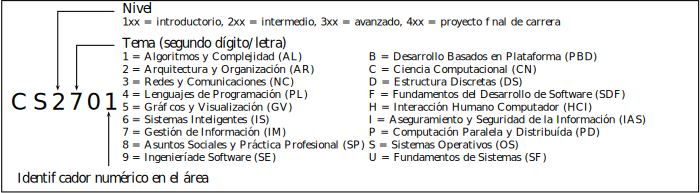
\includegraphics[width=13cm]{\OutputFigsDir/course-coding}
      \caption{Esquema de codificación para los cursos.}
      \label{fig:course-number}
      \end{figure}
\end{latexonly}
\begin{htmlonly}
      \begin{rawhtml}
            <p>
                  <img src="./figs/course-coding.png" style="width: 13cm; height: 5cm;">
            </p>
      \end{rawhtml}
\end{htmlonly}

El tipo de curso esta determinado por sus 2 primeras letras. Los posibles códigos para estos tipos son:
\input{\OutputTexDir/prefix-description}

Al mismo tiempo, y de acuerdo a la ley universitaria vigente, los cursos están clasificados en:
\begin{inparadesc}
\item [AF:] Área formativa,
\item [AE:] Área de especialidad,
\item [AB:] Área básica,
\item [AC:] Área complementaria.
\end{inparadesc}


% Table of courses by semesters
\begin{landscape}
\section{Estructura Curricular}\label{sec:courses-by-semester}
La relación de cursos se muestra a continuación:
\input{\OutputTexDir/tables-by-semester-\LANG}

\OnlySPC{Es importante resaltar que todos los semestres podrí­an ser completados con cursos extras de acuerdo al perfil de la institución.}
\end{landscape}



% \begin{landscape}
% \section{Distribución de tópicos por curso}\label{sec:topics-by-course}
Las siguientes tablas nos muestran la distribución de todos los tópicos del 
cuerpo del conocimiento de \ac{\currentarea} en todos los cursos.
\section{Distribución de tópicos por curso}\label{sec:topics-by-course}
Las siguientes tablas nos muestran la distribución de todos los tópicos del 
cuerpo del conocimiento de \ac{\currentarea} en todos los cursos.
\section{Distribución de tópicos por curso}\label{sec:topics-by-course}
Las siguientes tablas nos muestran la distribución de todos los tópicos del 
cuerpo del conocimiento de \ac{\currentarea} en todos los cursos.
\input{\OutputTexDir/topics-by-course}
% \end{landscape}

\begin{landscape}
\section{Resultados esperados distribuí­dos por curso}\label{sec:outcomes-by-course}
Las siquientes tablas nos muestras una visión global de los resultados que se esperan lograr en cada 
curso de la presente malla curricular. 
La lista completa de resultados esperados se encuentra en la Sección:~\ref{sec:outcomes}.
\input{\OutputTexDir/outcomes-by-course-\LANG}
\end{landscape}

\begin{landscape}
\section{Malla curricular}\label{sec:vision-grafica}
\vspace{-0.3cm}Este documento también puede ser analizado desde el punto de vista de los prerequisitos de forma gráfica.
\begin{figure}[h!]
      \includegraphics[width=23cm]{\OutputFigsDir/small-graph-curricula.ps}
      \label{fig:malla-curricular}
      \caption{Malla curricular \SchoolFullName}
\end{figure}
\end{landscape}

\section{Distribución de cursos en la carrera}
Esta propuesta puede ser analizada por el número de créditos dedicados a cada área
%horas de clase de las mismas
y por niveles de cursos (Introductorios, Intermedios, Avanzados y Proyectos).
\vspace{0.5cm}

\begin{figure}[h!]
      \centering
      \includegraphics[width=10cm]{\OutputFigsDir/pie-credits}
      \label{fig:pie-credits}
      \caption{Distribución de cursos por áreas considerando creditaje.}
\end{figure}

% \input{\OutputTexDir/distribution-area-by-semester}
\input{\OutputTexDir/distribution-credits-by-area-by-semester}

\begin{figure}[h!]
      \centering
      \includegraphics[width=10cm]{\OutputFigsDir/pie-by-levels}
      \label{fig:pie-niveles}
      \caption{Distribución de créditos por niveles de cursos.}
\end{figure} %Graphics by level, by area, etc

% \section{Compatibilidad de la carrera con relación a estandares internacionales}
% En esta sección presentamos la distribución de cursos por áreas de concentración en 
% contraste con las propuestas internacionales de las carreras de la \textit{Computing Curricula} 
% de \htmladdnormallink{IEEE-CS}{http://www.computer.org}/\htmladdnormallink{ACM}{http://www.acm.org}.
% 
% Es necesario notar que \underline{en algunos casos las materias podrían aparecen en más de un eje} 
% pues tienen contenido de más de una área. 
% Por ejemplo, la materia de sistemas operativos contiene unidades de aplicación 
% que pueden ser clasificadas en Tecnología de Información pero al mismo tiempo contiene fundamentos 
% de como está estructurado un Sistema Operativo que es del eje de Ciencia de la Computación. 
% En estos casos el creditaje ha sido divido entre los ejes correspondientes.
% \input{\OutputTexDir/list-of-courses-per-area}
% 
% Considerando esta distribución, las figuras \ref{fig:comparing-curves-\currentarea-\currentinstitution-with-CE} 
% a la \ref{fig:comparing-curves-\currentarea-\currentinstitution-with-SE} 
% nos permiten tener una visión gráfica de esta malla curricular frente a las propuestas de 
% carreras presentadas por \htmladdnormallink{IEEE-CS}{http://www.computer.org}/\htmladdnormallink{ACM}{http://www.acm.org} en la \textit{Computing Curricula}
% \input{\OutputTexDir/comparing-with-standards}
